\begin{figure}
\centering
%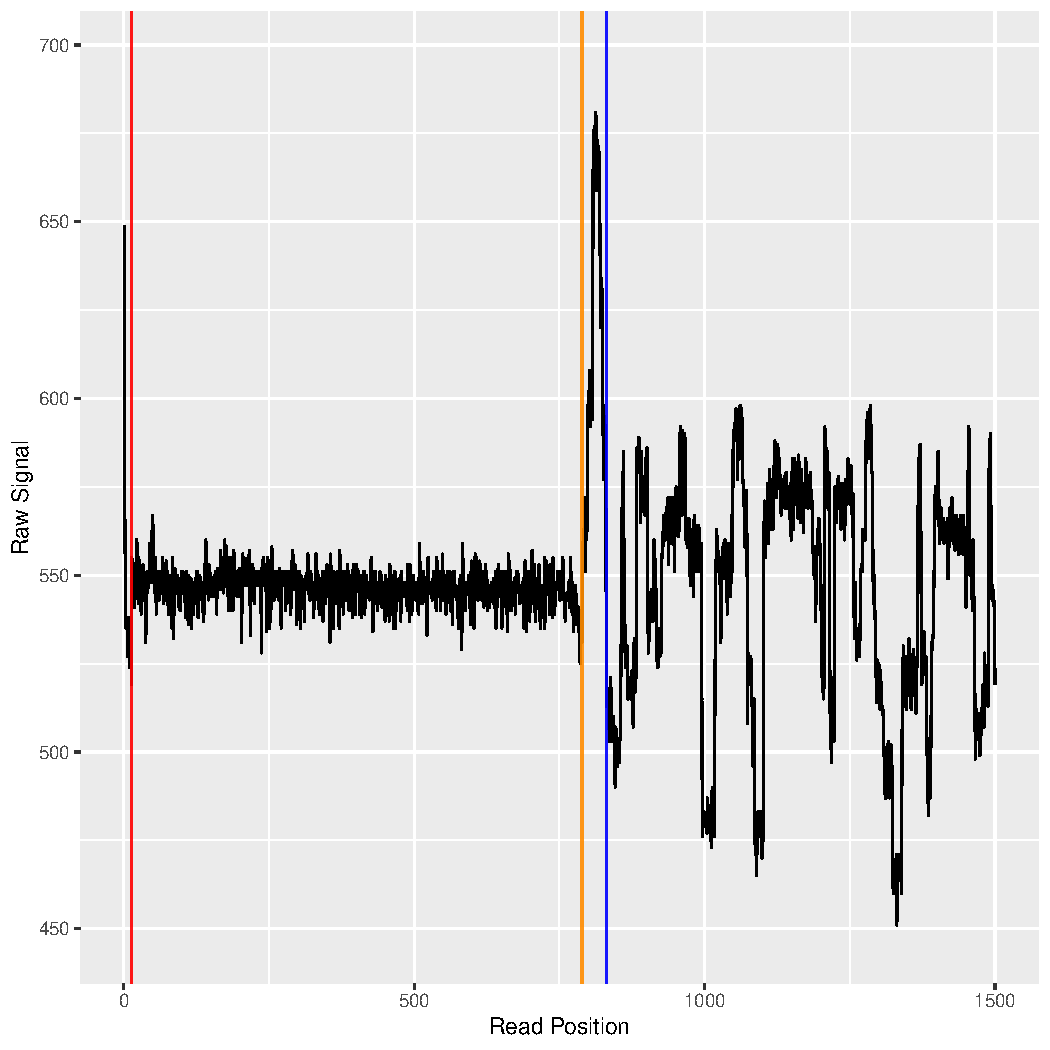
\includegraphics[scale=0.7]{plots/reads.e9f08690-171f-476f-9119-5330d0290126.raw.section.pdf}
% Created by tikzDevice version 0.12.3.1 on 2022-09-20 17:34:05
% !TEX encoding = UTF-8 Unicode
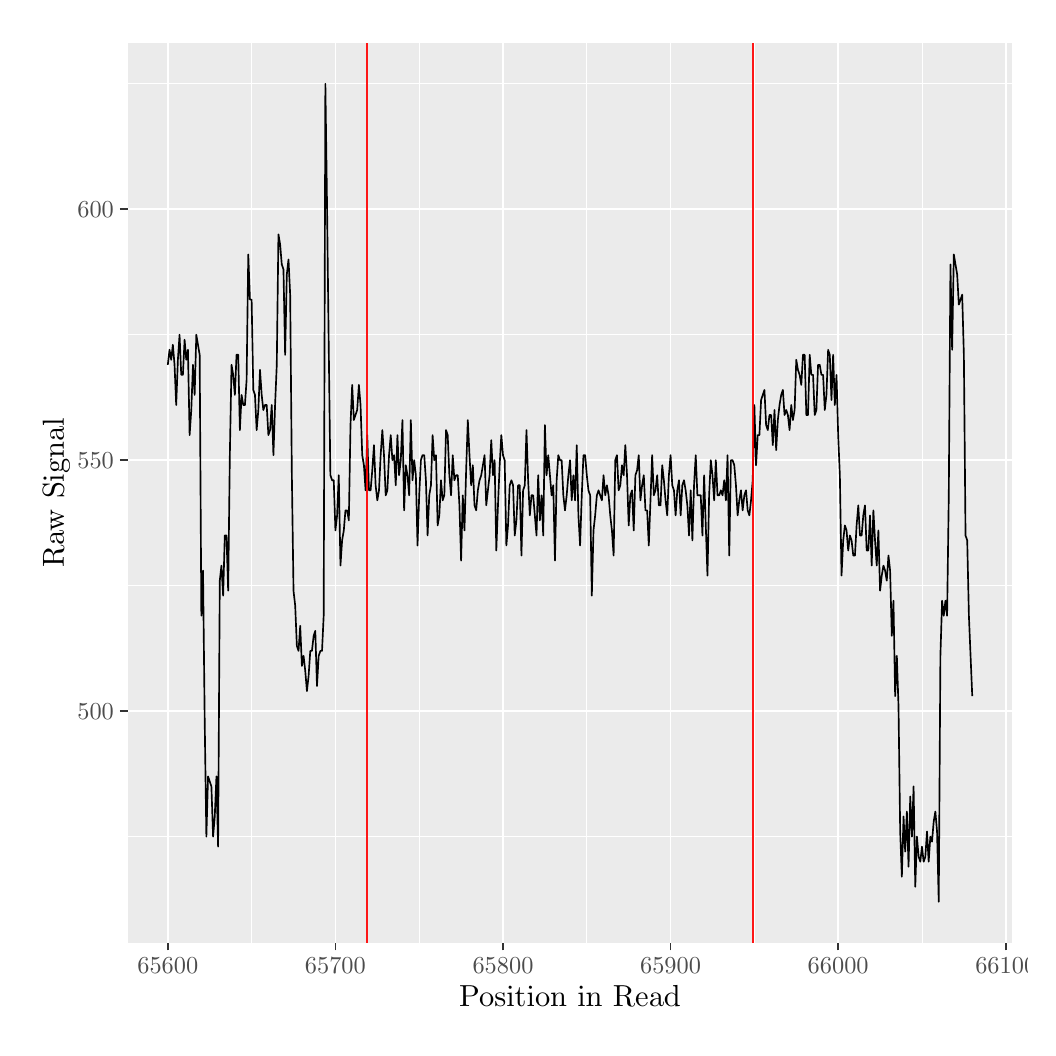
\begin{tikzpicture}[x=1pt,y=1pt]
\definecolor{fillColor}{RGB}{255,255,255}
\path[use as bounding box,fill=fillColor,fill opacity=0.00] (0,0) rectangle (361.35,361.35);
\begin{scope}
\path[clip] (  0.00,  0.00) rectangle (361.35,361.35);
\definecolor{drawColor}{RGB}{255,255,255}
\definecolor{fillColor}{RGB}{255,255,255}

\path[draw=drawColor,line width= 0.6pt,line join=round,line cap=round,fill=fillColor] (  0.00,  0.00) rectangle (361.35,361.35);
\end{scope}
\begin{scope}
\path[clip] ( 36.11, 30.69) rectangle (355.85,355.85);
\definecolor{fillColor}{gray}{0.92}

\path[fill=fillColor] ( 36.11, 30.69) rectangle (355.85,355.85);
\definecolor{drawColor}{RGB}{255,255,255}

\path[draw=drawColor,line width= 0.3pt,line join=round] ( 36.11, 69.04) --
	(355.85, 69.04);

\path[draw=drawColor,line width= 0.3pt,line join=round] ( 36.11,159.72) --
	(355.85,159.72);

\path[draw=drawColor,line width= 0.3pt,line join=round] ( 36.11,250.39) --
	(355.85,250.39);

\path[draw=drawColor,line width= 0.3pt,line join=round] ( 36.11,341.07) --
	(355.85,341.07);

\path[draw=drawColor,line width= 0.3pt,line join=round] ( 80.92, 30.69) --
	( 80.92,355.85);

\path[draw=drawColor,line width= 0.3pt,line join=round] (141.48, 30.69) --
	(141.48,355.85);

\path[draw=drawColor,line width= 0.3pt,line join=round] (202.04, 30.69) --
	(202.04,355.85);

\path[draw=drawColor,line width= 0.3pt,line join=round] (262.59, 30.69) --
	(262.59,355.85);

\path[draw=drawColor,line width= 0.3pt,line join=round] (323.15, 30.69) --
	(323.15,355.85);

\path[draw=drawColor,line width= 0.6pt,line join=round] ( 36.11,114.38) --
	(355.85,114.38);

\path[draw=drawColor,line width= 0.6pt,line join=round] ( 36.11,205.06) --
	(355.85,205.06);

\path[draw=drawColor,line width= 0.6pt,line join=round] ( 36.11,295.73) --
	(355.85,295.73);

\path[draw=drawColor,line width= 0.6pt,line join=round] ( 50.64, 30.69) --
	( 50.64,355.85);

\path[draw=drawColor,line width= 0.6pt,line join=round] (111.20, 30.69) --
	(111.20,355.85);

\path[draw=drawColor,line width= 0.6pt,line join=round] (171.76, 30.69) --
	(171.76,355.85);

\path[draw=drawColor,line width= 0.6pt,line join=round] (232.31, 30.69) --
	(232.31,355.85);

\path[draw=drawColor,line width= 0.6pt,line join=round] (292.87, 30.69) --
	(292.87,355.85);

\path[draw=drawColor,line width= 0.6pt,line join=round] (353.43, 30.69) --
	(353.43,355.85);
\definecolor{drawColor}{RGB}{0,0,0}

\path[draw=drawColor,line width= 0.6pt,line join=round] ( 50.64,239.51) --
	( 51.25,244.95) --
	( 51.86,241.33) --
	( 52.46,246.77) --
	( 53.07,239.51) --
	( 53.67,225.00) --
	( 54.28,241.33) --
	( 54.88,250.39) --
	( 55.49,235.89) --
	( 56.09,235.89) --
	( 56.70,248.58) --
	( 57.31,241.33) --
	( 57.91,244.95) --
	( 58.52,214.12) --
	( 59.12,223.19) --
	( 59.73,239.51) --
	( 60.33,228.63) --
	( 60.94,250.39) --
	( 61.54,246.77) --
	( 62.15,243.14) --
	( 62.76,148.84) --
	( 63.36,165.16) --
	( 63.97,110.75) --
	( 64.57, 69.04) --
	( 65.18, 90.80) --
	( 65.78, 88.99) --
	( 66.39, 87.18) --
	( 67.00, 69.04) --
	( 67.60, 76.30) --
	( 68.21, 90.80) --
	( 68.81, 65.41) --
	( 69.42,161.53) --
	( 70.02,166.97) --
	( 70.63,156.09) --
	( 71.23,177.85) --
	( 71.84,177.85) --
	( 72.45,157.90) --
	( 73.05,206.87) --
	( 73.66,239.51) --
	( 74.26,235.89) --
	( 74.87,228.63) --
	( 75.47,243.14) --
	( 76.08,243.14) --
	( 76.68,215.94) --
	( 77.29,228.63) --
	( 77.90,225.00) --
	( 78.50,225.00) --
	( 79.11,234.07) --
	( 79.71,279.41) --
	( 80.32,263.09) --
	( 80.92,263.09) --
	( 81.53,230.45) --
	( 82.13,228.63) --
	( 82.74,215.94) --
	( 83.35,223.19) --
	( 83.95,237.70) --
	( 84.56,228.63) --
	( 85.16,223.19) --
	( 85.77,225.00) --
	( 86.37,225.00) --
	( 86.98,214.12) --
	( 87.58,215.94) --
	( 88.19,225.00) --
	( 88.80,206.87) --
	( 89.40,225.00) --
	( 90.01,239.51) --
	( 90.61,286.66) --
	( 91.22,283.04) --
	( 91.82,275.78) --
	( 92.43,273.97) --
	( 93.03,243.14) --
	( 93.64,272.16) --
	( 94.25,277.60) --
	( 94.85,264.90) --
	( 95.46,199.62) --
	( 96.06,157.90) --
	( 96.67,152.46) --
	( 97.27,137.96) --
	( 97.88,136.14) --
	( 98.48,145.21) --
	( 99.09,130.70) --
	( 99.70,134.33) --
	(100.30,128.89) --
	(100.91,121.63) --
	(101.51,127.07) --
	(102.12,136.14) --
	(102.72,136.14) --
	(103.33,141.58) --
	(103.93,143.40) --
	(104.54,123.45) --
	(105.15,134.33) --
	(105.75,136.14) --
	(106.36,136.14) --
	(106.96,148.84) --
	(107.57,341.07) --
	(108.17,297.55) --
	(108.78,246.77) --
	(109.38,199.62) --
	(109.99,197.80) --
	(110.60,197.80) --
	(111.20,179.67) --
	(111.81,185.11) --
	(112.41,199.62) --
	(113.02,166.97) --
	(113.62,176.04) --
	(114.23,179.67) --
	(114.83,186.92) --
	(115.44,186.92) --
	(116.05,183.29) --
	(116.65,217.75) --
	(117.26,232.26) --
	(117.86,219.56) --
	(118.47,221.38) --
	(119.07,223.19) --
	(119.68,232.26) --
	(120.28,225.00) --
	(120.89,206.87) --
	(121.50,203.24) --
	(122.10,194.17) --
	(122.71,214.12) --
	(123.31,194.17) --
	(123.92,194.17) --
	(124.52,201.43) --
	(125.13,210.50) --
	(125.73,195.99) --
	(126.34,190.55) --
	(126.95,194.17) --
	(127.55,206.87) --
	(128.16,215.94) --
	(128.76,206.87) --
	(129.37,192.36) --
	(129.97,194.17) --
	(130.58,206.87) --
	(131.19,214.12) --
	(131.79,205.06) --
	(132.40,206.87) --
	(133.00,195.99) --
	(133.61,214.12) --
	(134.21,199.62) --
	(134.82,205.06) --
	(135.42,219.56) --
	(136.03,186.92) --
	(136.64,203.24) --
	(137.24,199.62) --
	(137.85,192.36) --
	(138.45,219.56) --
	(139.06,197.80) --
	(139.66,205.06) --
	(140.27,199.62) --
	(140.87,174.23) --
	(141.48,192.36) --
	(142.09,205.06) --
	(142.69,206.87) --
	(143.30,206.87) --
	(143.90,197.80) --
	(144.51,177.85) --
	(145.11,192.36) --
	(145.72,195.99) --
	(146.32,214.12) --
	(146.93,205.06) --
	(147.54,206.87) --
	(148.14,181.48) --
	(148.75,185.11) --
	(149.35,197.80) --
	(149.96,190.55) --
	(150.56,192.36) --
	(151.17,215.94) --
	(151.77,214.12) --
	(152.38,199.62) --
	(152.99,192.36) --
	(153.59,206.87) --
	(154.20,197.80) --
	(154.80,199.62) --
	(155.41,199.62) --
	(156.01,188.73) --
	(156.62,168.79) --
	(157.22,192.36) --
	(157.83,179.67) --
	(158.44,201.43) --
	(159.04,219.56) --
	(159.65,206.87) --
	(160.25,195.99) --
	(160.86,203.24) --
	(161.46,188.73) --
	(162.07,186.92) --
	(162.67,194.17) --
	(163.28,197.80) --
	(163.89,199.62) --
	(164.49,203.24) --
	(165.10,206.87) --
	(165.70,188.73) --
	(166.31,194.17) --
	(166.91,199.62) --
	(167.52,212.31) --
	(168.12,199.62) --
	(168.73,205.06) --
	(169.34,172.41) --
	(169.94,188.73) --
	(170.55,203.24) --
	(171.15,214.12) --
	(171.76,206.87) --
	(172.36,205.06) --
	(172.97,174.23) --
	(173.57,181.48) --
	(174.18,195.99) --
	(174.79,197.80) --
	(175.39,195.99) --
	(176.00,177.85) --
	(176.60,183.29) --
	(177.21,195.99) --
	(177.81,195.99) --
	(178.42,170.60) --
	(179.02,194.17) --
	(179.63,195.99) --
	(180.24,215.94) --
	(180.84,197.80) --
	(181.45,185.11) --
	(182.05,192.36) --
	(182.66,192.36) --
	(183.26,185.11) --
	(183.87,177.85) --
	(184.47,199.62) --
	(185.08,183.29) --
	(185.69,192.36) --
	(186.29,177.85) --
	(186.90,217.75) --
	(187.50,199.62) --
	(188.11,206.87) --
	(188.71,199.62) --
	(189.32,192.36) --
	(189.92,195.99) --
	(190.53,168.79) --
	(191.14,197.80) --
	(191.74,206.87) --
	(192.35,205.06) --
	(192.95,205.06) --
	(193.56,192.36) --
	(194.16,186.92) --
	(194.77,192.36) --
	(195.38,199.62) --
	(195.98,205.06) --
	(196.59,190.55) --
	(197.19,199.62) --
	(197.80,190.55) --
	(198.40,210.50) --
	(199.01,185.11) --
	(199.61,174.23) --
	(200.22,192.36) --
	(200.83,206.87) --
	(201.43,206.87) --
	(202.04,199.62) --
	(202.64,194.17) --
	(203.25,192.36) --
	(203.85,156.09) --
	(204.46,179.67) --
	(205.06,185.11) --
	(205.67,192.36) --
	(206.28,194.17) --
	(206.88,192.36) --
	(207.49,190.55) --
	(208.09,199.62) --
	(208.70,192.36) --
	(209.30,195.99) --
	(209.91,192.36) --
	(210.51,185.11) --
	(211.12,179.67) --
	(211.73,170.60) --
	(212.33,205.06) --
	(212.94,206.87) --
	(213.54,194.17) --
	(214.15,195.99) --
	(214.75,203.24) --
	(215.36,199.62) --
	(215.96,210.50) --
	(216.57,199.62) --
	(217.18,181.48) --
	(217.78,192.36) --
	(218.39,194.17) --
	(218.99,179.67) --
	(219.60,199.62) --
	(220.20,201.43) --
	(220.81,206.87) --
	(221.41,190.55) --
	(222.02,195.99) --
	(222.63,199.62) --
	(223.23,186.92) --
	(223.84,186.92) --
	(224.44,174.23) --
	(225.05,190.55) --
	(225.65,206.87) --
	(226.26,192.36) --
	(226.86,194.17) --
	(227.47,199.62) --
	(228.08,188.73) --
	(228.68,188.73) --
	(229.29,203.24) --
	(229.89,197.80) --
	(230.50,190.55) --
	(231.10,185.11) --
	(231.71,199.62) --
	(232.31,206.87) --
	(232.92,195.99) --
	(233.53,194.17) --
	(234.13,185.11) --
	(234.74,194.17) --
	(235.34,197.80) --
	(235.95,185.11) --
	(236.55,195.99) --
	(237.16,197.80) --
	(237.76,194.17) --
	(238.37,188.73) --
	(238.98,177.85) --
	(239.58,194.17) --
	(240.19,176.04) --
	(240.79,195.99) --
	(241.40,206.87) --
	(242.00,192.36) --
	(242.61,192.36) --
	(243.21,192.36) --
	(243.82,177.85) --
	(244.43,199.62) --
	(245.03,181.48) --
	(245.64,163.34) --
	(246.24,192.36) --
	(246.85,205.06) --
	(247.45,199.62) --
	(248.06,190.55) --
	(248.66,205.06) --
	(249.27,192.36) --
	(249.88,192.36) --
	(250.48,194.17) --
	(251.09,192.36) --
	(251.69,197.80) --
	(252.30,190.55) --
	(252.90,206.87) --
	(253.51,170.60) --
	(254.11,205.06) --
	(254.72,205.06) --
	(255.33,203.24) --
	(255.93,195.99) --
	(256.54,185.11) --
	(257.14,190.55) --
	(257.75,194.17) --
	(258.35,186.92) --
	(258.96,192.36) --
	(259.57,194.17) --
	(260.17,186.92) --
	(260.78,185.11) --
	(261.38,190.55) --
	(261.99,197.80) --
	(262.59,225.00) --
	(263.20,203.24) --
	(263.80,214.12) --
	(264.41,214.12) --
	(265.02,226.82) --
	(265.62,228.63) --
	(266.23,230.45) --
	(266.83,217.75) --
	(267.44,215.94) --
	(268.04,221.38) --
	(268.65,221.38) --
	(269.25,210.50) --
	(269.86,223.19) --
	(270.47,208.68) --
	(271.07,219.56) --
	(271.68,225.00) --
	(272.28,228.63) --
	(272.89,230.45) --
	(273.49,221.38) --
	(274.10,223.19) --
	(274.70,221.38) --
	(275.31,215.94) --
	(275.92,225.00) --
	(276.52,219.56) --
	(277.13,223.19) --
	(277.73,241.33) --
	(278.34,237.70) --
	(278.94,235.89) --
	(279.55,232.26) --
	(280.15,243.14) --
	(280.76,243.14) --
	(281.37,221.38) --
	(281.97,221.38) --
	(282.58,243.14) --
	(283.18,235.89) --
	(283.79,235.89) --
	(284.39,221.38) --
	(285.00,223.19) --
	(285.60,239.51) --
	(286.21,239.51) --
	(286.82,235.89) --
	(287.42,235.89) --
	(288.03,223.19) --
	(288.63,228.63) --
	(289.24,244.95) --
	(289.84,243.14) --
	(290.45,226.82) --
	(291.05,243.14) --
	(291.66,225.00) --
	(292.27,235.89) --
	(292.87,214.12) --
	(293.48,199.62) --
	(294.08,163.34) --
	(294.69,176.04) --
	(295.29,181.48) --
	(295.90,179.67) --
	(296.50,172.41) --
	(297.11,177.85) --
	(297.72,176.04) --
	(298.32,170.60) --
	(298.93,170.60) --
	(299.53,181.48) --
	(300.14,188.73) --
	(300.74,177.85) --
	(301.35,177.85) --
	(301.95,185.11) --
	(302.56,188.73) --
	(303.17,172.41) --
	(303.77,172.41) --
	(304.38,185.11) --
	(304.98,166.97) --
	(305.59,186.92) --
	(306.19,176.04) --
	(306.80,166.97) --
	(307.40,179.67) --
	(308.01,157.90) --
	(308.62,163.34) --
	(309.22,166.97) --
	(309.83,165.16) --
	(310.43,161.53) --
	(311.04,170.60) --
	(311.64,165.16) --
	(312.25,141.58) --
	(312.85,154.28) --
	(313.46,119.82) --
	(314.07,134.33) --
	(314.67,116.19) --
	(315.28, 70.86) --
	(315.88, 54.53) --
	(316.49, 76.30) --
	(317.09, 63.60) --
	(317.70, 78.11) --
	(318.30, 58.16) --
	(318.91, 83.55) --
	(319.52, 69.04) --
	(320.12, 87.18) --
	(320.73, 50.91) --
	(321.33, 69.04) --
	(321.94, 61.79) --
	(322.54, 59.97) --
	(323.15, 65.41) --
	(323.76, 59.97) --
	(324.36, 61.79) --
	(324.97, 70.86) --
	(325.57, 59.97) --
	(326.18, 69.04) --
	(326.78, 67.23) --
	(327.39, 74.48) --
	(327.99, 78.11) --
	(328.60, 70.86) --
	(329.21, 45.47) --
	(329.81,134.33) --
	(330.42,154.28) --
	(331.02,148.84) --
	(331.63,154.28) --
	(332.23,148.84) --
	(332.84,192.36) --
	(333.44,275.78) --
	(334.05,244.95) --
	(334.66,279.41) --
	(335.26,275.78) --
	(335.87,272.16) --
	(336.47,261.27) --
	(337.08,263.09) --
	(337.68,264.90) --
	(338.29,243.14) --
	(338.89,177.85) --
	(339.50,176.04) --
	(340.11,148.84) --
	(340.71,134.33) --
	(341.32,119.82);
\definecolor{drawColor}{RGB}{255,0,0}

\path[draw=drawColor,draw opacity=0.90,line width= 0.6pt,line join=round] (122.71, 30.69) -- (122.71,355.85);

\path[draw=drawColor,draw opacity=0.90,line width= 0.6pt,line join=round] (261.99, 30.69) -- (261.99,355.85);
\end{scope}
\begin{scope}
\path[clip] (  0.00,  0.00) rectangle (361.35,361.35);
\definecolor{drawColor}{gray}{0.30}

\node[text=drawColor,anchor=base east,inner sep=0pt, outer sep=0pt, scale=  0.88] at ( 31.16,111.35) {500};

\node[text=drawColor,anchor=base east,inner sep=0pt, outer sep=0pt, scale=  0.88] at ( 31.16,202.03) {550};

\node[text=drawColor,anchor=base east,inner sep=0pt, outer sep=0pt, scale=  0.88] at ( 31.16,292.70) {600};
\end{scope}
\begin{scope}
\path[clip] (  0.00,  0.00) rectangle (361.35,361.35);
\definecolor{drawColor}{gray}{0.20}

\path[draw=drawColor,line width= 0.6pt,line join=round] ( 33.36,114.38) --
	( 36.11,114.38);

\path[draw=drawColor,line width= 0.6pt,line join=round] ( 33.36,205.06) --
	( 36.11,205.06);

\path[draw=drawColor,line width= 0.6pt,line join=round] ( 33.36,295.73) --
	( 36.11,295.73);
\end{scope}
\begin{scope}
\path[clip] (  0.00,  0.00) rectangle (361.35,361.35);
\definecolor{drawColor}{gray}{0.20}

\path[draw=drawColor,line width= 0.6pt,line join=round] ( 50.64, 27.94) --
	( 50.64, 30.69);

\path[draw=drawColor,line width= 0.6pt,line join=round] (111.20, 27.94) --
	(111.20, 30.69);

\path[draw=drawColor,line width= 0.6pt,line join=round] (171.76, 27.94) --
	(171.76, 30.69);

\path[draw=drawColor,line width= 0.6pt,line join=round] (232.31, 27.94) --
	(232.31, 30.69);

\path[draw=drawColor,line width= 0.6pt,line join=round] (292.87, 27.94) --
	(292.87, 30.69);

\path[draw=drawColor,line width= 0.6pt,line join=round] (353.43, 27.94) --
	(353.43, 30.69);
\end{scope}
\begin{scope}
\path[clip] (  0.00,  0.00) rectangle (361.35,361.35);
\definecolor{drawColor}{gray}{0.30}

\node[text=drawColor,anchor=base,inner sep=0pt, outer sep=0pt, scale=  0.88] at ( 50.64, 19.68) {65600};

\node[text=drawColor,anchor=base,inner sep=0pt, outer sep=0pt, scale=  0.88] at (111.20, 19.68) {65700};

\node[text=drawColor,anchor=base,inner sep=0pt, outer sep=0pt, scale=  0.88] at (171.76, 19.68) {65800};

\node[text=drawColor,anchor=base,inner sep=0pt, outer sep=0pt, scale=  0.88] at (232.31, 19.68) {65900};

\node[text=drawColor,anchor=base,inner sep=0pt, outer sep=0pt, scale=  0.88] at (292.87, 19.68) {66000};

\node[text=drawColor,anchor=base,inner sep=0pt, outer sep=0pt, scale=  0.88] at (353.43, 19.68) {66100};
\end{scope}
\begin{scope}
\path[clip] (  0.00,  0.00) rectangle (361.35,361.35);
\definecolor{drawColor}{RGB}{0,0,0}

\node[text=drawColor,anchor=base,inner sep=0pt, outer sep=0pt, scale=  1.10] at (195.98,  7.64) {Position in Read};
\end{scope}
\begin{scope}
\path[clip] (  0.00,  0.00) rectangle (361.35,361.35);
\definecolor{drawColor}{RGB}{0,0,0}

\node[text=drawColor,rotate= 90.00,anchor=base,inner sep=0pt, outer sep=0pt, scale=  1.10] at ( 13.08,193.27) {Raw Signal};
\end{scope}
\end{tikzpicture}

\caption{\label{fig:homo-section}An example of a homopolymer section (repetition of `T') from the read with ID e9f08690-171f-476f-9119-5330d0290126. The thymine DNA base is repeated 33 times in the homopolymer.}
\end{figure}
